\documentclass[12pt]{article}
\usepackage{graphicx}
\usepackage{amsmath}
\usepackage{amssymb}
\usepackage{amsthm} 
\usepackage[T1]{fontenc}
\usepackage[francais]{babel}
\usepackage[utf8]{inputenc}
\usepackage{enumerate}
\usepackage{ifpdf}
\usepackage{color} 
\usepackage[top=2.0cm,right=2.0cm,bottom=3.1cm,left=2.5cm]{geometry}
\usepackage{fancyhdr}
\usepackage{eso-pic}
\usepackage{hyperref}
\usepackage{longtable}
\usepackage{graphicx}
\usepackage{verbatim}
\usepackage{listings}
\usepackage{wrapfig}
%configuration de listings
	%definition de couleurs 
	\definecolor{colKeys}{rgb}{0.16,0.5,0.16}
	\definecolor{colIdentifier}{rgb}{0,0,0}
	\definecolor{colComments}{rgb}{0,0,1}
	\definecolor{colString}{rgb}{0.8,0.3,0.3}
	\lstset{%configuration de listings
		float=hbp,%
		basicstyle=\ttfamily\footnotesize, %
		identifierstyle=\color{colIdentifier}, %
		keywordstyle=\color{colKeys} \bf, %
		stringstyle=\color{colString}, %
		commentstyle=\color{colComments}, %
		backgroundcolor=\color{white},
		%columns=flexible, %
		tabsize=4, %
		frame=lrTB, % cadre
		frameround=tttt, % bord du cadre arondis
		extendedchars=true, %
		showspaces=false, %
		showstringspaces=false, %
		numbers=left, %
		numberstyle=\tiny, %
		stepnumber=1, %
		breaklines=true, % pour que les lignes trop longues dans les programmes ne debordent pas
		breakautoindent=true, %
		captionpos=b,%
	}
	
% configuration du style de la page
\pagestyle{fancy}
\fancyhead[LO,LE]{
\includegraphics[height=9.0mm]{img/logo.png}}
\fancyfoot{}
\fancyfoot[RE,RO]{\thepage\AddToShipoutPicture*{
\includegraphics[width=\paperwidth,height=30.0mm]{img/Volutes3_v3.jpg}}}
\fancypagestyle{plain}{% 1ères pages des chapitres
	\fancyhead{}
	\fancyfoot{}
	\fancyhead[LO,LE]{
\includegraphics[height=9.0mm]{img/logo.png}}
	%\fancyfoot[RE,RO]{\thepage\AddToShipoutPicture*{
\includegraphics[width=\paperwidth,height=30.0mm]{img/Volutes3_v3.jpg}}}
}

%opening
\title{Guide d'utilisation de wordpress}
\author{Yicheng GAO}
\date{Ao\^ut 2012}

\begin{document}

\maketitle



\section{Le site de management du wordpress}
Pour accéder au site de management de wordpress de windeo Green Futur : \\
\url{http://www.windeo-planet.com/wordpress/wp-admin}\\

\subsection{L'onglet \texttt{Pages}}
Vous voyez une liste des onglets à gauche, les différents pages sont stockés dans l'onglet «Pages». Si vous voulez ajouter une page (un formulaire par exemple), il faut cliquer «Ajouter» en haut du «Pages»
\begin{figure}[!htbp]
\centering

\includegraphics[scale=0.5]{img/1}
\end{figure}

\subsection{L'onglet \texttt{Formulaire}}
Les détails du formulaire sont stocké en onglet "Formulaire"
\begin{figure}[!htbp]
\centering
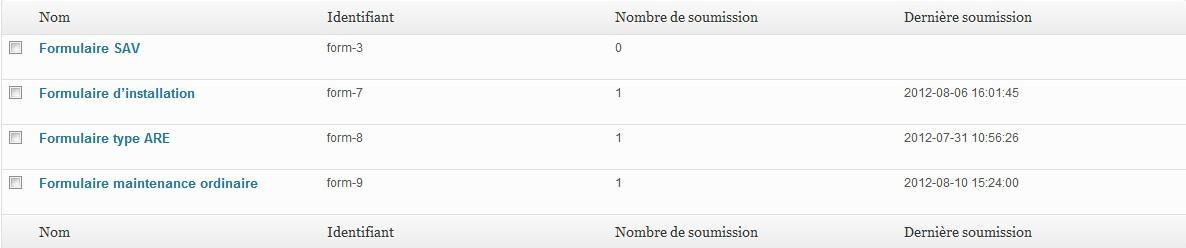
\includegraphics[width=\textwidth]{img/2}
\end{figure}
\newpage
Pour rappel, les identifiants de chaque formulaire (form-3 par exemple) est identique que celui dans le «Pages», et aussi identique avec le nom du tableau pour la base de donnée.

\begin{figure}[!htbp]
\centering
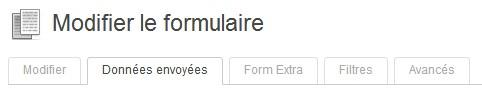
\includegraphics[scale=0.7]{img/3}
\end{figure}

Les données sont stockés dans l’onglet ‘Données envoyées’, on détaillera cette partie dans la section \texttt{3.Base de Donnée}.


\section{Modifier du formulaire}
Si vous avez besoin de modifier le formulaire, vous allez dans onglet Formulaire, et cliquer sur ‘Modifier’

\begin{figure}[!htbp]
\centering

\includegraphics[width=\textwidth]{img/4}
\end{figure}

Vous pouvez voir les différents types de choix au-dessus dont vous pouvez les ajouter dans le formulaire

\begin{figure}[!htbp]
\centering
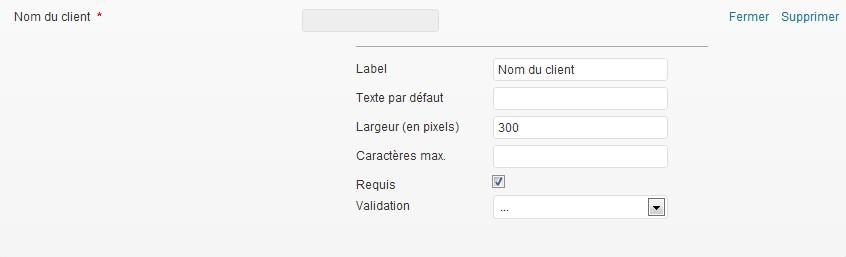
\includegraphics[width=\textwidth]{img/5}
\end{figure}

Pour chaque ligne du formulaire, on peut les modifier(changement du label, ajouter l’option de validation, etc.) ou supprimer


\section{Base de donnée}
Il y a 3 façons pour manipuler la base de donnée de wordpress:
\begin{itemize}
\item l'outil \texttt{Formulaire} du wordpress(méthode principale)
\item l'extension \texttt{Database Browser}
\item logiciel \texttt{phpMyAdmin}
\end{itemize}
\subsection{L'outil \texttt{Formulaire} du wordpress}
C'est la méthode principale pour visualiser les données du formulaire, vous connectez d'abord sur le wordpress avec le login et mot de passe d'admin, puis vous cliquez le bouton \texttt{Formulaire} à gauche, vous choississez le formulaire concerné, et puis l'onglet \texttt{Donneés envoyées} en haut, 
\begin{figure}[!htbp]
\centering
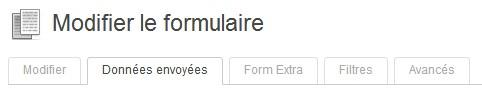
\includegraphics[scale=0.7]{img/3}
\end{figure}

Dans le page \texttt{Données envoyées}, vous pouvez visualiser la totalité des données, faire la recherche, trier, supprimer les données et télécharger sous format plain texte.

\subsection{L'extension \texttt{Database Browser}}
C'est une extension intergré dans wordpress,vous allez sur l'onglet \texttt{Outils} à gauche, puis \texttt{Database Browser}.\\

Ensuite vous choississez le tableau concerné, et puis vous pouvez visualiser les données et télécharger sous 4 formes: XML, HTML, CSV, JSON.\\

Rappel: Les identificateurs de chaque colonne ne conforme pas avec les noms des lables, c'est parce que les identificateurs sont només par wordpress automatiquement, qui ne peuvent pas changés. 

\begin{figure}[!htbp]
\centering
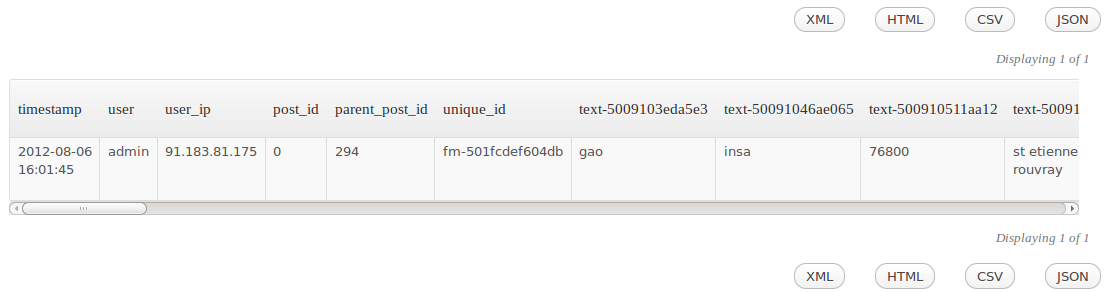
\includegraphics[scale=0.4]{img/14}
\end{figure}



\subsection{Logiciel \texttt{phpMyAdmin}}

PhpMyAdmin (PMA) est une application Web de gestion pour les systèmes de gestion de base de données MySQL réalisée en PHP et distribuée sous licence GNU GPL.\\

\begin{figure}[!htbp]
\centering
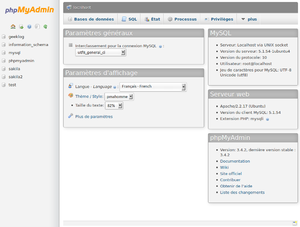
\includegraphics[scale=1]{img/13}
\end{figure}

Il s'agit de l'une des plus célèbres interfaces pour gérer une base de données MySQL sur un serveur PHP. De nombreux hébergeurs, qu'ils soient gratuits ou payants, le proposent ce qui permet à l'utilisateur de ne pas avoir à l'installer.\\

Cette logiciel est installé déjà sur le serveur FTP avec l'adresse d'emplacement:\\ \texttt{ftp://178.208.41.22/httpdocs/www/phpMyAdmin}\\

Vous pouvez accéder au gestionnaire de la base de donnée avec \\
\url{http://www.windeo-planet.com/phpMyAdmin/}
Avec le login et mot de passe de de base de donnée wordpress.

\begin{figure}[!htbp]
\centering
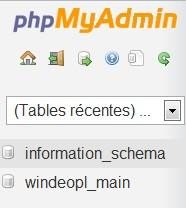
\includegraphics[scale=0.8]{img/6}
\end{figure}

Dans la page d’accueil, vous pouvez voir 2 tableaux \texttt{information\_schema} et \texttt{windeopl\_main}, les informations concernant le formulaire sont stockés dans le tableau \texttt{windeopl\_main}

\begin{figure}[!htbp]
\centering
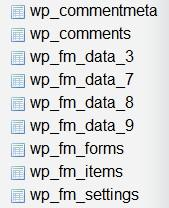
\includegraphics[scale=1]{img/7}
\end{figure}

Les données des formulaires sont nommés \texttt{wp\_fm\_data\_NUM}
Pour chaque formulaire, il y a une liste des onglets au-dessus:

\begin{figure}[!htbp]
\centering

\includegraphics[width=\textwidth]{img/8}
\end{figure}

\begin{itemize}
\item[Afficher:] Affichage la totalité des données du formulaire\\

\item[Structure:] Les différents lignes du formulaire, on peut changer les nom, mais attention, une fois le nom est changé, on ne peut pas accéder au «données envoyées» dans wordpress, c’est parce que les noms sont données par wordpress et ne peuvent pas touchés.\\

\item[SQL:] faire le recherche ou modification par le code sql\\

\item[Recherche:] faire la recherche par interface graphique\\

\item[Exporter:] Pour exporter les données du formulaire,  il y a plusieurs formats à choisir\\

\item[Rappel:] Les identifiant du données ne sont pas identique du label dans le formulaire, c’est parce que ces nom sont donnés par wordpress dirtement, qui ne peuvent pas changer.
\end{itemize}


\begin{figure}[!htbp]
\centering
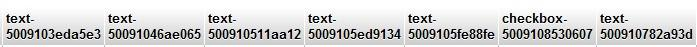
\includegraphics[width=\textwidth]{img/9}
\end{figure}

Un tutoriel complèt: \url{http://www.siteduzero.com/tutoriel-3-14496-phpmyadmin.html}

\section{Autres fonctionnalités du wordpress}
\subsection{Changement du mot de passe du «news FTP»}
Pages-News FTP-Visibilité en haut à droite
\begin{figure}[!htbp]
\centering
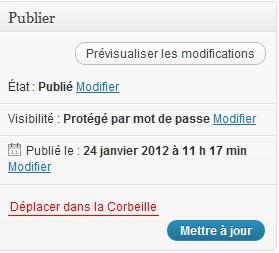
\includegraphics[scale=0.7]{img/10}
\end{figure}
\subsection{La notification par mail}
Réglages – SMTP\\
Dans la page de configation SMTP, il faut remplir les informations concernant le serveur mail, après on peut faire une test pour voir si ça marche.\\

Maintenant la fonction de la notification par mail ne marche pas, car le serveur a interdit les ports concernés (SMTP par exemple). 
\begin{figure}[!htbp]
\centering
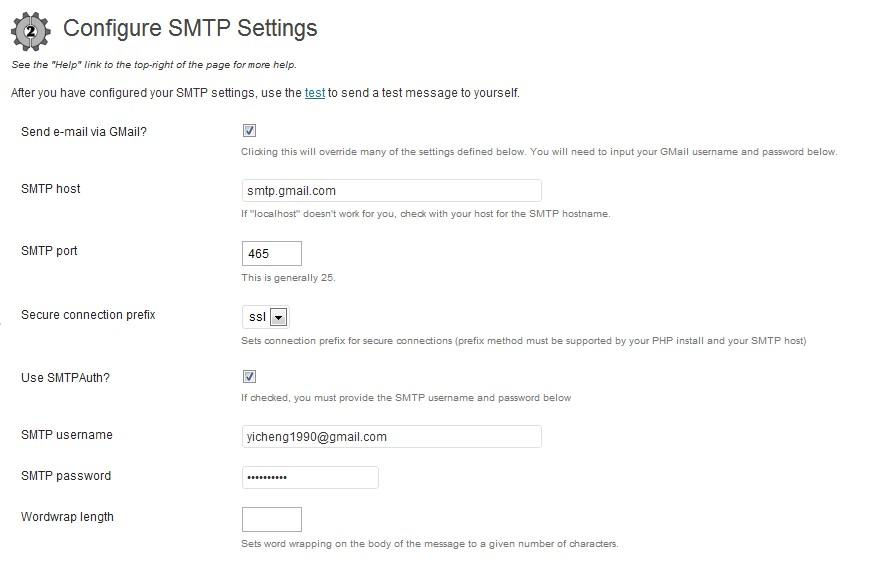
\includegraphics[scale=0.5]{img/11}
\end{figure}

\newpage
\subsection{Changement du mot de passe d'accès du wordpress}

Pour changer le mot de passe d'accès du wordpress, il faut aller au \\ \texttt{ftp://178.208.41.22/httpdocs/www/wordpress/login.php} et changer la deuxième ligne:
\begin{verbatim}
$password = 'XXXX';
\end{verbatim}\\

Pour supprimer la fonction d'authentification, il faut supprimer les codes suivantes dans le fichier: \\ \texttt{ftp://178.208.41.22/httpdocs/www/wordpress/wp-content/themes/twentyten/header.php} (Sachant que le thème utilisé est \texttt{twentyten})\\


\begin{verbatim}
  session_start();
    if( isset($_SESSION['authenticated']) )
    {
        if($_SESSION['authenticated'] == 'yes')
        {
            $authenticated = 'yes';
        }
        else
        {
            $authenticated = 'no';
        }
    }
    else
    {
        $authenticated = 'no';
    }

    if($authenticated != 'yes')
    {
        header("Location: http://www.windeo-planet.com/wordpress/login.php");
        exit();
    }
\end{verbatim}


\section{l'outil pour l'échange des fichiers FTP}

\url{http://filezilla-project.org/}\\

FileZilla est un client FTP. Un logiciel libre qui vous permet de charger ou télécharger les fichiers sur un serveur. Par exemple les éléments de votre site web chez ou depuis votre hébergeur. Il possède une interface utilisateur graphique intuitive. Rapide et fiable, Filezilla est gratuit et multi-plateforme : il fonctionne sur tout système d’exploitation. Supporte plusieurs types de connexion : client FTP, FTPS et SFTP (mode normal ou sécurisé). Indispensable à tous ceux qui gèrent un site Web ou envisagent de le faire.\\

\begin{figure}[!htbp]
\centering
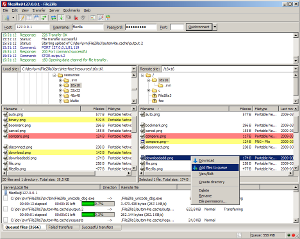
\includegraphics[scale=1.2]{img/12}
\end{figure}

Vous pouvez connecter au serveur FTP avec login et mot de passe de Windeo en haut, la boite à gauche est l'emplacement des fichiers local, la boite à droite est celui des fichiers FTP.Vous pouvez faire la syntonisation avec les opérations simples.\\

Le site de téléchargement: \url{http://filezilla-project.org/download.php/}, avec votre type de OS\\

\section{L'outil pour faire la synchronisation des fichier FTP}

\url{http://www.goodsync.com/}

GoodSync est un logiciel de synchronisation de fichiers et de sauvegarde de fichiers qui opère automatiquement les syncs entre PC de bureau, portables et disques externes.\\

Il y a des tutoriels complèts sur le site.

\begin{figure}[!htbp]
\centering
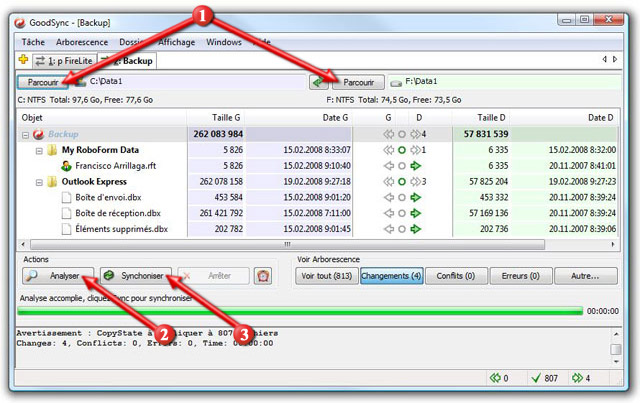
\includegraphics[scale=0.7]{img/15}
\end{figure}


\end{document}
